\cleardoublepage %poner esta linea al inicio de cada capitulo

\chapter{Introducción}

La agricultura ha sido uno de los pilares más importantes tanto para el desarrollo de la sociedad como para su manutención, ya que es gracias a está, que los países pueden generar empleos y aumentar sus recursos económicos, sin embargo las tareas de agricultura pueden llegar a ser tediosas o muy pesadas para las personas, es por esto que con el avance tecnológico se ha buscado mejorar el sector agricultor no solo para facilitar a los agricultores las tareas que deben hacer, sino también permitir que el producto que están ofreciendo sea de mayor calidad, para garantizar que su comercialización tenga un mayor auge globalmente.
\\
La visión artificial se ha implementado en el sector agricultor para corregir las fallas humanas y garantizar que el producto mantenga siempre una buena calidad, ya que para poder exportar productos agrícolas estos deben estar bajo los requisitos de las normas INCONTEC.
\\
Este proyecto busca implementar mediante un proceso mecatrónico las técnicas de visión artificial para ayudar al crecimiento del sector papicultor en Colombia, el cual se ha visto afectado por los tratados de libre comercio establecidos por el gobierno nacional. 


\newpage
\section{Objetivos}

\subsection{Objetivo General}

Proponer un prototipo para la clasificación de características de calidad en los tubérculos de papa producidos en la región Andina de Colombia, mediante técnicas de visión por computadora.

\subsection{Objetivos Específicos}
\begin{enumerate}
	\item Identificar a través de técnicas de visión artificial los rasgos de calidad "y características físicas" que se encuentran en los tubérculos de papa. 
	\item Evaluar el desempeño del prototipo propuesto para realizar la clasificación de los tubérculos de papa bajo la norma NTC341. 
	\item Comparar la precisión del modelo propuesto con modelos similares de clasificación
\end{enumerate}

\section{Alcances y Limitaciones}

\subsection{Alcances}

Para la realización del proyecto se debe tener en cuenta que se enfocará en los tubérculos de papa tipo pastusa producidos en la región andina de Colombia, los cuales se deben encontrar lavados para llevar acabo un análisis más preciso, el análisis estará enfocado en identificar las características de calidad del producto predicho para ser comercializado. Ádemas de esto el prototipo propuesto será de ayuda únicamente en el desplazamiento del producto para su análisis. 

\subsection{Limitaciones}


El proyecto se encuentra limitado a los recursos de software y hardware (computacionales) con los que cuentan los integrantes del proyecto y las plataformas open sources que se le puedan sacar provecho para la implementación de los algoritmos que actualmente se encuentran en la literatura. Por otro lado se presentan limitaciones para la construcción del elemento por la contingencia sanitaria presentada hoy en día, los procesos de mecanizados como lo son el torno, la fresadora y la soldadura de la universidad se encuentran limitados por la contingencia.


\section{Justificación}
El presente proyecto implementará técnicas de visión artificial en el sector papicultor colombiano con el fin de comprobar la eficacia de la clasificación de calidad en los tubérculos de papa, ya que Actualmente, el cultivo de la papa constituye el eje fundamental de la economía del país en 283 municipios a nivel nacional, donde se involucran más de 90.000 familias principalmente en los departamentos de Boyacá, Cundinamarca, Antioquia y Nariño, los cuales concentran más del 85 \% de la producción \cite{referencia1}.
Actualmente el reto que enfrenta el sector es el aumento de la calidad del producto, el rendimiento en producción y en consecuencia, incrementar el consumo. Debido a que la producción de papa en Colombia aporta el 3.3 \% del Producto Interno Bruto (PIB) agropecuario, las siembras son de alrededor de 130 mil hectáreas y se cosechan cerca de 2,8 millones de toneladas, Además, en Colombia la producción de papa genera anualmente alrededor de 264.000 empleos, aproximadamente 75.000 son trabajos directos y alrededor de 189.000 son indirectos \cite{referencia2}
Así el presente trabajo permitirá mostrar los beneficios que trae la implementación de técnicas de visión artificial permitiendo un crecimiento al sector papicultor y aumentando la calidad del producto para que pueda ser comercializado tanto a nivel local como global.


\section{Descripción y formulación del problema}
La agricultura de Colombia es un componente fundamental en la economía del territorio, Juega un papel primordial en el desarrollo económico del país. Debido a que es la principal fuente de ingresos del área rural, hace un aporte relevante al desarrollo económico, la mitigación de la pobreza, y el desarrollo sustentable de Colombia. Uno de los sectores más   grandes en la agricultura colombiana es el sector papicultor, en Colombia se caracteriza por tener poco desarrollo tecnológico y buscar abastecer el consumo interno, sin mayor exploración en mercados internacionales. Frente a la coyuntura en la que se encuentra el sector gracias a los retos que trae consigo los acuerdos comerciales firmados por el gobierno nacional, el sector papicultor requiere urgentes transformaciones que permitan aumentar su competitividad y por ende lograr el crecimiento del sector.
Como consecuencia en los últimos años el sector agricultor de Colombia ha implementado herramientas tecnológicas que le permitan a los agricultores aumentar la calidad de sus productos y así poder competir tanto en el mercado local como en el global. Pensando en esto las diferentes técnicas de visión artificial han tenido un auge en la agricultura de precisión ayudando a clasificar productos basándose en sus diferentes características sin importar su clase, sin embargo, las técnicas de visión artificial no han sido aprovechadas para mejorar el sector papicultor colombiano.
El sector agricultor de Colombia ha implementado diferentes técnicas de visión artificial las cuales ayudan a clasificar los productos mediante las características que estos poseen, sin embargo no se ha implementado estas técnicas en la fase de almacenamiento de los tubérculos de papa, la cual es importante ya que en esta fase es donde se separan los tubérculos que cumplen las condiciones de calidad de los tubérculos que se encuentran defectuosos, ya que para la comercialización de este producto deben estar clasificados según la norma NTC 341.\\ 

¿Cómo se puede aumentar la eficiencia al clasificar los tubérculos de papa bajo la norma NTC341 mediante técnicas de visión artificial para su distribución comercial?\\

¿Qué tipo de proceso de clasificación permitirá agrupar los tubérculos de papa según sus características físicas y "patologías" mediante técnicas de visión artificial?	


\chapter{Estado del arte}

\section{MatLab.}
	El objetivo de los antecedentes es analizar y realizar una revisión literaria sobre lo  que  se  ha hecho  a  nivel  teórico  y  práctico  en  cuanto a  la visión artificial en agricultura de precisión.  Además,  determinar  cuáles son los aportes que éstos le puedan dar a este trabajo de investigación.\\
	
	Comenzando por la literatura con temática en el procesamiento de imágenes se tiene el artículo \cite{article3}, en donde se menciona que la implementación de MATLAB\textsuperscript{\textregistered} como una herramienta de procesamiento de imágenes, radica en su facilidad para realizar cambios a las imágenes, es por esto qué diseñó un sistema para la clasificación de objetos en base a su forma y color usando métodos de visión artificial en MATLAB\textsuperscript{\textregistered} con el uso de la librería \textit{ufm.dll} para capturar y procesar imágenes. El artículo \cite{inproceedings} presenta una investigación en dónde se consiguió calcular el tamaño de diferentes mangos estimando el área cubierta en una imagen binaria (imagen digital que tiene únicamente dos valores posibles para cada píxel) con base al número de píxeles, luego de ser procesadas las imágenes, se clasificaron implementando un algoritmo basado en \textit{fuzzy logic} teniendo en cuenta 5 variedades diferentes de mangos y como referencias el color de la cascara, tamaño, defectos superficiales, forma, firmeza, peso y olor.\\

\section{Artificial Neural Networks.}
	En cuanto a la clasificación, se deben usar técnicas de visión artificial y en primer lugar, se revisó literatura  acerca de ANN (\textit{Artificial Neural Networks}) como el articulo \cite{article2} en el Perú  aplicó visión artificial usando ANN como método de clasificación de las principales características extraídas de las frutas, que son derivadas del análisis de las superficies tanto en su contenido cromático como en la cantidad y distribución de defectos externos. De igual forma, en el trabajo \cite{Shrivastava2017}, presentaron un sistema de visión artificial que usa un enfoque de categorización simplificado con un elevado índice de exactitud. El propósito del sistema es clasificar los granos de trigo de las especies \textit{triticum aestivum} y \textit{triticum durum} según sus propiedades visuales usando una ANN del tipo MLP (\textit{Multilayer Perceptron}); las imágenes se obtienen por medio de una cámara que captura las propiedades de tamaño, color y textura de cada grano con el objeto de que sirvan de acceso al procedimiento de categorización. Otro trabajo es \cite{Singh2016}, quien propone el uso de redes neuronales BPNN (\textit{Back Propagation Artificial Neural Networks}) como método de clasificación y la descomposición mediante ondículas (Tipo especial de transformada matemática que representa una señal en términos de versiones trasladadas y dilatadas de una onda finita) para clasificar los granos de arroz. El modelo de clasificación implemento una red neuronal BPNN de cuatro capas la cual presento mejores resultados en comparación con otros métodos.\\
	
	Por último, usando el método de clasificación ANN, se tiene el artículo \cite{Przybyl2019} presenta un trabajo para garantizar la correcta clasificación de los productos y reducir las pérdidas durante su almacenamiento. La investigación abarca esfuerzos centrados en la evaluación sensorial de patatas con el análisis de imágenes por ordenador y la modelización neuronal ANN. El objetivo de este estudio fue desarrollar un método para asistir a la identificación de cualquiera de las variedades y la turgencia de los tubérculos de patata(Fenómeno que ocurre cuando una célula se dilata debido a la presión ejercida por los fluidos y por el contenido celular sobre las paredes de la célula) llevado a cabo sobre la base de los datos gráficos codificados en forma de imágenes digitales, obtenidos mediante algoritmos que interpretan los descriptores de imagen.\\

\section{Super Vector Machine.}
	Otro método de clasificación revisado en la literatura es el de SVM \textit{Super Vector Machine}), como el usado en el trabajo \cite{LIU201679}, en donde realizaron un proceso para analizar granos de arroz. El procedimiento usa 4 fuentes de luz para crear la sombra del grano en 4 direcciones; la diferencia en medio de las siluetas de los granos llenos y no llenos se evalúan por medio del estudio de imágenes y un clasificador SVM. El análisis se hace mediante el uso de imágenes RGB (Red-Green-Blue) de los granos con las siluetas, luego se segmentan por  desde la imagen binaria, para sustraer información como el sector del grano y de la sombra. En el documento \cite{CHUNG2016404} se menciona un método para clasificar plántulas (Embrión ya desarrollado como consecuencia de la germinación de una semilla) sanas e infectadas. Consiste en el análisis de imágenes mediante un escáner y el proceso de clasificación utilizando SVM, en donde se hace uso de dos clasificadores, el primero distingue entre las plantas sanas y contaminadas, por otra parte, el segundo mide los niveles de contaminación. En el trabajo \cite{PIRES201648} se propuso un método de detección automática de enfermedad en cultivos de soja, el cual se basa en descripciones locales conocido como el método BOV (Bag of Values) luego de escanear la hoja. Se obtuvo a través de los vectores de entrada una clasificación en dos categorías, enfermo y sano, a partir de un clasificador SVM. Y por último, en este tipo de clasificador, el documento \cite{SUN2014426} propone un sistema para analizar el porcentaje de granos en el arroz que se encuentran en condiciones para ser distribuidos. El algoritmo se encarga de la división de los granos de manera automática. Tras la segmentación, es viable obtener el número de granos presentes en la imagen y la información específica, la exactitud del procedimiento puede verse afectada si el germen no se extrae del todo por esa razón el sistema detecta la viable región de germen y estima esta información usando SVM.\\

\section{Otros métodos.}
	En la literatura se encontraron artículos que usaban más de un método de clasificación, un ejemplo es \cite{LIU201682} que puso en práctica un método para controlar la población de pulgones (Familia de insectos hemípteros) en el trigo, usando los métodos SVM, el algoritmo MSER (\textit{Maximally Stable Extremal Regions}), y el HOG (\textit{Histogram of Gradients}).El uso de estos 3 métodos se conoce como SMH (Unión entre SVM, MSER y HOG, que se basa en el análisis de imágenes, tratadas a partir de unos parámetros con la finalidad de detectar la presencia y/o ausencia de pulgones, se hizo uso de este método a partir del color y la densidad de población. Al comparar este método con otros cinco comúnmente utilizados, los resultados presentaron un rendimiento superior en la identificación de pulgones. \\
	
	De igual manera, el artículo \cite{sobolu2020automatic} propone un algoritmo de clasificación automática de patatas. Se Realizó dos tipos de clasificación: una en función del tamaño de las patatas y otra en función de su calidad. La segmentación de las zonas defectuosas se hizo mediante métodos como \textit{global thresholding} para extraer \textit{morphological and statistical features} de las zonas segmentadas. Estas características se eligieron como entradas para los algoritmos de clasificación, en donde se usaron los métodos SVM, \textit{Decision  Tree} y LDA (\textit{Linear Discriminant Analysis}) implementados en MATLAB\textsuperscript{\textregistered} Classification Toolbox.Se llegó a la conclusión de que la SVM ha clasificado las patatas según su tamaño con una mayor tasa de éxito. En el caso de la clasificación por calidad, se recomienda el método LDA.\\
	
	Los anteriores son los métodos más comunes que se encontraron en la literatura investigada, sin embargo, hay unos métodos poco comunes como por ejemplo los presentados en el artículo \cite{article5} en donde se identificó objetos en movimiento mediante la ayuda de la visión artificial y la transmisión de datos a un brazo robótico implementando \textit{C++} y \textit{Open CV} usando el código de cadena (Actualmente el grupo de reconocimiento de patrones e inteligencia artificial aplicada) para calcular las características de los objetos por color y forma. También, el artículo \cite{7237209} que se usa para la detección automática, fue necesario hacer uso inicialmente de separar el fondo de la hoja, para este proceso se usó el algoritmo MCW (\textit{Marker-Controlled Watershed}), el SLIC (\textit{Simple Linear Iterative Clustering}) se utilizó para obtener las características presentadas por la enfermedad sobre la planta y por ultimo para la clasificación y textura se obtienen a través de GLCM (\textit{Gray Level Co-occurrence Matrix}), el modelo de clasificación fue el SVM, este método propuesto presento un mayor rendimiento.\\
	
	Y el último artículo revisado es el \cite{Barnes2010}, cuyo objetivo de  investigación es introducir un método automático de detección de manchas en imágenes digitales de patatas. El sistema desarrollado es entrenable, de modo que pueda trabajar con diferentes variedades de patatas y variaciones en las estaciones, condiciones de iluminación, etc. Otro objetivo, pensando en su posible implantación en entornos industriales, es permitir el procesamiento de imágenes en tiempo real, posiblemente mediante la construcción de \textit{Minimalist Boosted Classifier} que extraigan un subconjunto mínimo de todas las características que optimicen el rendimiento de la detección con el menor coste computacional posible.


\chapter{Marco Conceptual}

	\subsection{\textbf{Agricultura de precisión:}} El término sobre el que se inspira la agricultura de precisión es utilizar la porción adecuada de insumos, en el instante correcto y en el sitio preciso. La agricultura de precisión (AP) implica la utilización de sistemas de posicionamiento universal (GPS) y de otros medios electrónicos para obtener datos del cultivo. Las tecnologías de la agricultura de precisión permiten saciar una de las exigencias de la agricultura actualizada: el funcionamiento óptimo de enormes extensiones. Se muestra como primordial virtud que la exploración de resultados de los ensayos se puede hacer por sectores diferentes en un mismo lote, y tal cual ajustar el desempeño diferencial en los mismos. La utilización de las tecnologías de la agricultura de precisión puede contribuir a mejorar los márgenes, por medio de un incremento del costo del rendimiento (cantidad o calidad), de una reducción en la proporción de insumos, o de los dos paralelamente.
	\\
	\subsection{\textbf{Artificial Neural Networks:}} Las RNA son sistemas de procesamiento de la información cuya composición y manejo permanecen inspirados en las redes neuronales biológicas. Consisten en un enorme conjunto de recursos básicas de procesamiento denominados nodos o neuronas que permanecen organizados en capas. De esta forma, las RNA son sistemas adaptativos que aprenden de la vivencia, en otros términos, aprenden a realizar ciertas labores por medio de un entrenamiento con ejemplos ilustrativos.
	\\ 
	
	\subsection{\textbf{Imagen Binaria:}} La binarización de una imagen se apoya en un proceso de reducción de la información de la misma, en la que únicamente persisten 2 valores: verdadero y falso. En el proceso y estudio de imagen, la binarización se emplea para dividir las zonas u objetos de interés en una imagen del resto. En otras ocasiones, una imagen binaria es sencillamente el resultado de una selección interactiva de zonas de interés, las cuales se usarán como máscaras de comparación o alusión.
	\\ 
	
	\subsection{\textbf{ISO 800:}} ISO no es más que la sensibilidad del sensor en el momento de captar la luz. A más grande número de ISO, más grande capacidad para captar luz, a menor costo, menor capacidad para capturar esa luz. Una vez que duplicas el costo ISO, o sea, pasas de, ejemplificando, ISO 100 a ISO 200, necesitas la mitad de luz para poder hacer la misma exposición.
	\\ 
	
	\subsection{\textbf{Procesamiento de imagenes:}} El procesamiento de imágenes tiene como fin mejorar el aspecto de las imágenes y hacer más evidentes en ellas ciertos detalles que se quieren hacer percibir. La imagen puede haber sido generada de muchas posibilidades, ejemplificando, fotográficamente, o electrónicamente, mediante monitores de televisión. El procesamiento de las imágenes se puede generalmente hacer mediante procedimientos ópticos, o bien mediante procedimientos digitales, en una PC. En la siguiente parte describiremos bastante brevemente dichos 2 procedimientos, sin embargo, previamente se va a hacer una síntesis brevísima de los principios matemáticos implícitos en los dos procedimientos, donde el teorema de Fourier es el eje central.
	\\ 
	
	\subsection{\textbf{Reconstrucción morfológica:}} La recomposición morfológica se puede tener en cuenta conceptualmente como dilataciones reiteradas de una imagen, denominadas, hasta que el contorno de la imagen del marcador se adapta bajo una segunda imagen, llamada imagen de máscara En la recomposición morfológica, los picos de la imagen del marcador "se alargan" o se dilatan.
	\\ 
	
	\subsection{\textbf{Tubérculos de papa:}} La papa o patata es un tubérculo que se puede comer que se extrae de la planta herbácea americana Solanum tuberosum, de procedencia andino. Es una planta correspondiente a el núcleo familiar de las solanáceas procedente de Suramérica y cultivada por todo el planeta por sus tubérculos víveres. Ha sido domesticada en el altiplano andino por sus pobladores entre el 8500 y el 5000 a. n. e., y después ha sido llevada a Europa por los colonizadores españoles como una curiosidad botánica más que como una planta alimenticia. Su consumo ha sido creciendo y su cultivo se expandió a todo el planeta hasta transformarse actualmente en uno de los más importantes alimentos para la gente.
	\\ 
	
	\subsection{\textbf{Visión artificial:}} La perspectiva artificial ayuda a la industria a mejorar los procesos de producción por medio de imágenes digitales, con ellas se optimiza el control de calidad de aplicaciones industriales y de robots. Los sistemas de perspectiva examinan y se aseguran de conseguir los requisitos mínimos de calidad exigidos por cada fabricante. A lo largo del proceso de inspección los sistemas de perspectiva informan de los probables errores detectados, lo cual posibilita un mejor control del proceso de producción.






\chapter{Dataset Tubérculos de papas}


\section{Creación del Dataset}
	Las fotos tomadas para la creacion del \textit{Dataset} poseen un tamaño de (3168, 4752) pixeles. Fueron tomadas con una cámara profesional \textit{Canon EOS 50D} que tiene 15.1 mega pixeles de resolución y se puede ajustar la sensibilidad ISO desde 100 a 3200. La cámara fue configurada con ISO-800 que corresponde al parámetro de sensibilidad del sensor de ruido de la cámara, una velocidad de obturación de $\frac{1}{640}$ segundos que corresponde al dispositivo que controla el tiempo en el que la luz incide sobre el sensor de la cámara y finalmente una apertura de diafragma de $F7.1$ que corresponde a la apertura del lente que deja pasar la luz \cite{Camara}, tener en cuenta que a mayor F, menor luz se deja pasar. Se construyó una caja con iluminación fija usando bombillos de luz blanca de 6500 Kelvin de temperatura de color para que la iluminación en todas las fotos tomadas fuera uniforme:

	\begin{figure}[ht]
		\centering
		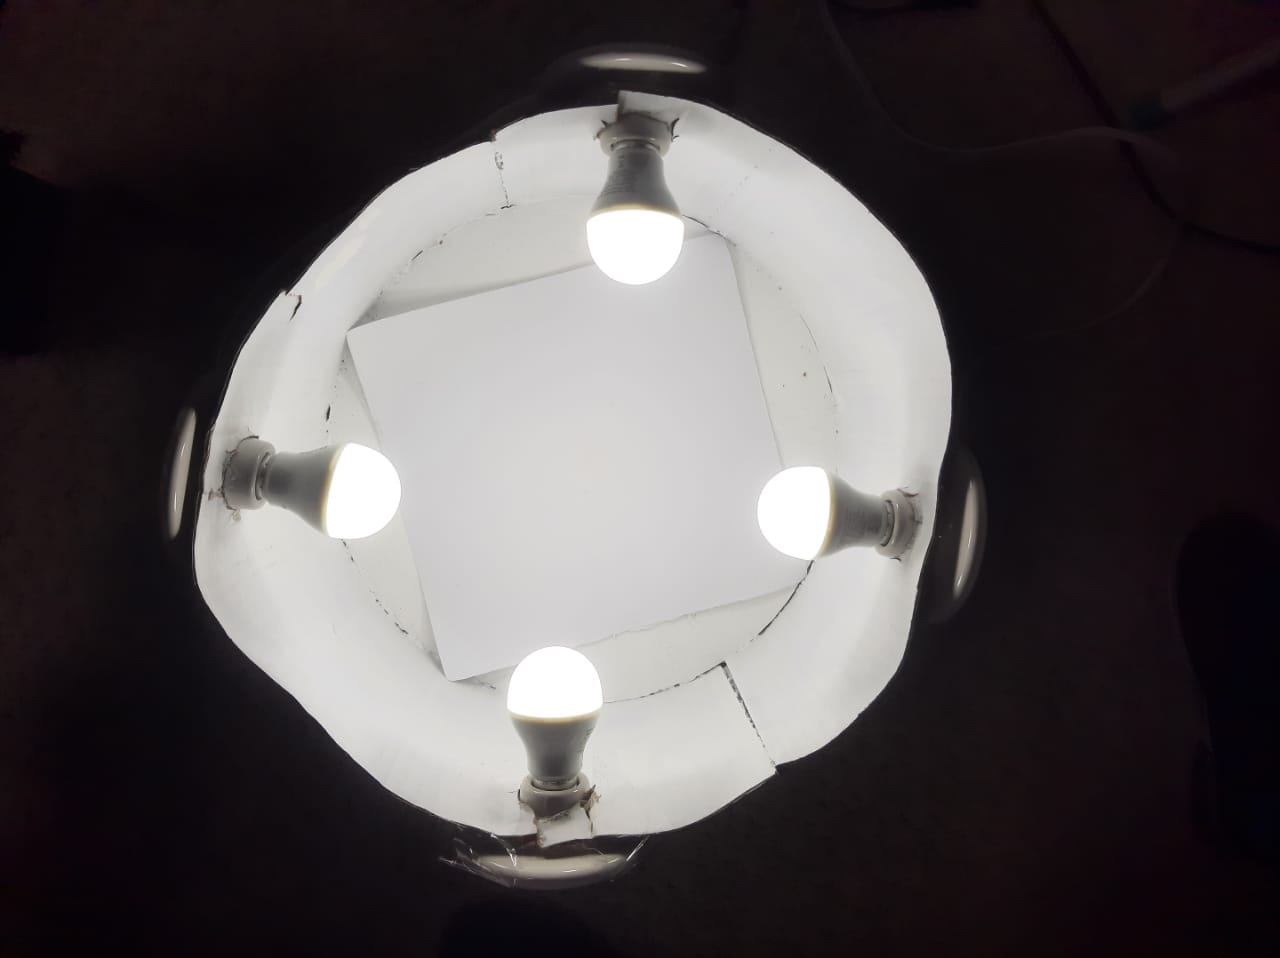
\includegraphics[scale=0.2]{Figs/Chamber.JPEG}
		\caption{Caja para tomar fotos}
		\label{fig:chamber}
	\end{figure}

\newpage
	Se creó un \textit{dataset} de 592 imágenes de papa tipo R12 y tipo pastusa las cuales se implementarán para train y para test además de 75 imágenes de tuberculos para la comprobación del algoritmo. Se realizará una clasificación en tres categorias que son, tipo, daño y tamaño. Las etiquetas de cada imagen se encuentran dentro del nombre de cada archivo, de la siguiente manera:

	\begin{itemize}
		\item $[Tipo]$ es 0(Pastusa) y 1(R12).
		\item $[Dano]$ es 0(Buena) y 1(Defectuosa).
		\item $[Tamano]$ de 0 a 2 corresponde a muy grande, grande y mediana.
		\item $[Numero \ de \ la \ imagen]$ etiqueta asignada por la cámara.
	\end{itemize}

	Ejemplo clasificación de imagenes:
	
	\begin{table}[ht]
		\centering
		\begin{tabular}{|c|c|c|c|}
			\hline
			TIPO & DAÑO & TAMAÑO & FILENAME \\
			\hline
			R12 & DEFECTUOSA & GRANDE & 1\_1\_1\_075.JPG \\
			\hline
			PASTUSA & BUENA & GRANDE & 0\_0\_1\_1973.JPG \\
			\hline
			R12 & BUENA & GRANDE & 1\_0\_1\_2054.JPG \\
			\hline
			PASTUSA & BUENA & MEDIANA & 0\_0\_2\_2042.JPG \\
			\hline
			PASTUSA & BUENA & GRANDE & 0\_0\_1\_1955.JPG \\
			\hline
		\end{tabular}	
		\caption{MetaData}
		\label{table:metadata}
	\end{table}

	En la tabla podemos apreciar la distribución del \textit{MetaData} de las imagenes almacendas en el \textit{Dataset}, donde se toman cinco imagenes al azar. A partir de esta tabla se crea un archivo \textit{.CSV} donde se encuentra la informacion de las 592 imagenes.




\newpage

\section{Distribución del Dataset}

	Se presenta la distribución del dataset segun las categorias establecidas.  
	
	\begin{table}[ht]
		\centering
		\begin{tabular}{|c|c|c|c|c|}
			\hline
			PASTUSA & R12 & BUENA & DEFECTUOSA & CLASE \\
			\hline
			X &  & X &  & CLASE 1 \\
			\hline
			X &  &  & X & CLASE 2 \\
			\hline
			  & X & X &  & CLASE 3 \\
			\hline
			  & X &  & X & CLASE 4 \\
			\hline
		\end{tabular}	
		\caption{Clases}
		\label{table:Clases}
	\end{table}
	  
	Los Datasets de \textit{Train} y \textit{Test} son creados para el entrenamiento y validacion de la red neuronal, programada para la clasificacion de imagenes, estos son separados en $80\%$ para \textit{Train} y $20\%$ para \textit{Test}. Se crearon archivos \textit{.CSV}, como se mostro en la tabla \ref{table:metadata}, los cuales contienen el metadata y la direccion de las imagenes por separado. De esta manera obtenemos la clasificacion del dataset segun el metadata de sus imagenes.
	
	\begin{figure}[ht]
		\centering
		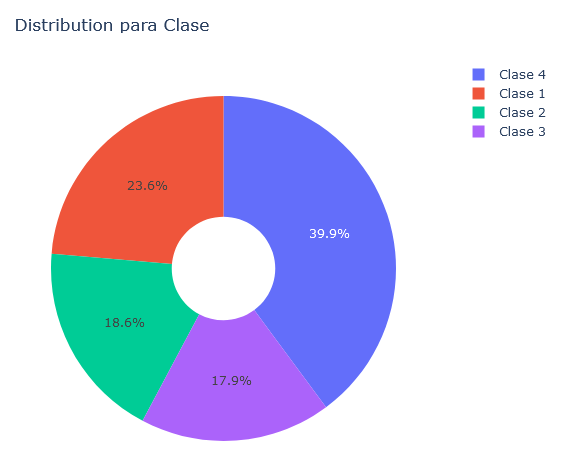
\includegraphics[scale=0.6]{Figs/4.png}
		\caption{Distribución del Dataset segun las categorias}
		\label{fig:distribucion}
	\end{figure}


\newpage
\chapter{Algoritmo de clasificación}

	\section{Red neuronal artificial}

		\subsection{Data Augmentation}
			\subsubsection{Definición}
			\subsubsection{Preprocesamiento de imagenes}
			funcion pytorch.compose
			\subsubsection{Filtro Gaussiano}

		\subsection{Datasets y DataLoaders}
			\subsubsection{Función Dataset}
			explicar funcion atributos y transform
			\subsubsection{Función Dataloader}
			batch size shuffle y num of workers
		
		\subsection{Hiperparámetros del modelo}
			\subsubsection{Stride and Padding and maxpooling and activation funtion}
			\subsubsection{Dropout}
			\subsubsection{Función de perdidas}
			incluir parte matematica?
			\subsubsection{Optimizador}
			momentum y learning rate
			\subsubsection{Backward pero otro nombre}
			xxx
			
		\subsection{Optimización Bayesiana}	
			
			
		\subsection{Arquitectura del modelo}
			\subsubsection{Modelo preentrenado ALEXNET}
			\subsubsection{Modelo preentrenado RESNET18}
			\subsubsection{Modelo preentrenado VGG19}
			\subsubsection{Modelo preentrenado VGG11}
			\subsubsection{Comparación de arquitecturas}
		
	\section{Clasificación de tamaño}
	
\chapter{Prototipo}
	

	















